% !TEX encoding = UTF-8 Unicode

\documentclass[a4paper]{article}

\usepackage{color}
\usepackage{url}
\usepackage[T2A]{fontenc} 
\usepackage[utf8]{inputenc}
\usepackage{graphicx}

\usepackage[english,serbian]{babel}
\usepackage[unicode]{hyperref}
\hypersetup{colorlinks,citecolor=red,filecolor=green,linkcolor=blue,urlcolor=blue}

\begin{document}

\title{Bezbednost na internetu i etičko hakovanje\\ \small{Seminarski rad u okviru kursa\\Računarstvo i društvo\\ Matematički fakultet}}

\author{Nemanja Lisinac\\ nemanjalisinac@gmail.com}
\date{28.~april 2022.}
\maketitle

\abstract{
Ovaj rad se bavi terminima bezbednosti na internetu ({\em Cybersecurity})  i njegovom podgranom Etičko hakovanje. Obrađeni su osnovni principi cybersecuritija, sta je to u suštini, kao i osvrt na to šta je etičko hakovanje, čime se bavi i različiti tipovi hakera. 

\tableofcontents

\newpage

\section{Cybersecurity i istorijat sistema}
\label{sec:uvod}
Sigurno ste primetili da kada hoćete da resetujete vašu šifru, internet stranica prvo mora da potvrdi vaš identitet i tek nakon dokaza da je to baš vaš nalog, možete promeniti šifru. To je jedna od stvari kojima se bavi cyber security.

Pod pojmom cyber security smatramo primenu tehnologija, procesa i pravila kako bi zaštitili sisteme, mreže, uređaje i podatke od hakerskih napada. To se postiže kombinacijom alata koji omogućavaju što veću sigurnost i smanjuju šansu od potencijalnih napada. 

Neki od različitih tipova napada na internetu su:
\begin{itemize}
\item \textbf{Zlonamerni programi ({\em Malware})} - kao što su programi koji traže otkup {\em ransomware},  dozvoljavaju pristup {\em RAT - remote access tools}, trojanci {\em Trojan viruses}...
\item \textbf{DDos napadi ({\em Distributed denial-of-service})} - napadi na internet tačke gde je u cilju preopterećenje i skidanje tačke sa interneta
\item \textbf{DNS napadi ({\em Domain name system})} - promene u provajderu ip adresa na osnovu naziva stranica i time se korisnik može proslediti na bilo koji sajt
\item \textbf{Kripto majneri ({\em Cryptojacking})} - instaliranje kripto majnera na uređaj
\end{itemize}
\cite{whatiscybersec}

Skoro svaki sistem može biti žrtva napada na internetu, a hakerima najinteresantniji su svakako finansijski sistemi zbog mogućnosti zarade. Tako da su nebrojano puta bile hakovane velike finansijske institucije poput SWIFT-a, investicionih banaka i slično. Takođe, sajtovi i aplikacije koji dozvoljavaju plaćanje i čuvanje podataka o karticama su na meti, zbog lakog prebacivanja novca, ostvarivanja kupovina na drugim sajtovima kao i prodaje podataka na crnom tržistu.

Od pojave interneta, sa razvojem digitalizacije, pojam{\em cybersecurity} postaje sastavni deo ličnog i poslovnog života. 70- tih godina, uglavnom je bio rezervisan samo za ljude koji su se time bavili, sve do masovnog širenja interneta, gde se sa povećanjem ''povezanosti'' povećava i mogućnost napada. Tada nije bilo nekih velikih pretnji jer su kompjuteri i internet bili u razvoju i lako je bilo pronaći bezbednosne propuste. Najčešći napadi tada su bili tako što čovek iznutra pristupi poverljivom dokumentu. 
1971. godine se pojavio prvi virus nazvan{\em Creeper}. Napravio ga je Bob Thomas i smatra se prvim kompjuterskim crvom.
Godinu dana kasnije je razvijen prvi antivirusni program nazvan {\em Reaper}. Napravljen od strane Ray Tomlinson, on je mogao da se kreće kroz tadašnju internet mrežu ({\em ARPANET}) i da pronalazi i uništava virus {\em Creeper}. 
Između 1986. i 1987. godine, grupa nemačkih hakera je izvela prvi zabeležen slučaj internet špijunaže. Oni su upali u sisteme američke bezbednosti, fakulteta i vojnih baza i prikupili informacije koje su prodali KGB-u.
1988. se desio napad koji je privukao veliku pažnju tadašnjih medija. Virus koji je nazvan {\em Morris worm} se proširio internetom. Napravio ga je student koji je kasnije uhvaćen i to je prvi slučaj koji je završio na sudu.\cite{computersecurity}


\newpage

\section{Faze cybersecuritija}
\label{sec:faze}
Kako bi se zaštitili od napada, ceo proces je podeljen na 4 faze: 
\begin{itemize}
\item \textbf{Identifikacija} - treba videti koji delovi su rizični i rangirati ih. U to ne spada samo fizička infrastruktura, već i procesi kroz koje ljudi imaju interakciju sa tom infrastrukturom.
\item \textbf{Zaštita} - zaštititi delove koji su rizični. Najnovije verzije korišćene tehnologije i njihova redovna nadogradnja su najbolji način da se brzo i jednostavno reše potencijalne sigurnosne brige. Takođe pojedini uređaji imaju mogućnost samonadogradnje, gde se mogu nadograditi automatski bez interakcije sa korisnikom.
\item \textbf{Detekcija} - saznati da se desio sigurnosni proboj. Mrežni log fajlovi i sistemi za nadgledanje mreže omogućavaju kompanijama da nadgledaju tok podataka i neautorizovane pristupe mreži. Detekcioni sistem takođe treba da ima mogućnost uzbune i slanja izveštaja. 
\item \textbf{Reakcija} - reagovati na detektovan sigurnosni proboj i ako je naneta šteta, ispraviti je. Najvažniji deo oporavka u slučaju napada je zaštita informacija od značaja. Treba preduzeti mere koje će sprečiti budući napad uz što manji uticaj na normalan rad uređaja.
\end{itemize} \cite{cyberphases}

\begin{figure}[h!]
	\begin{center}
		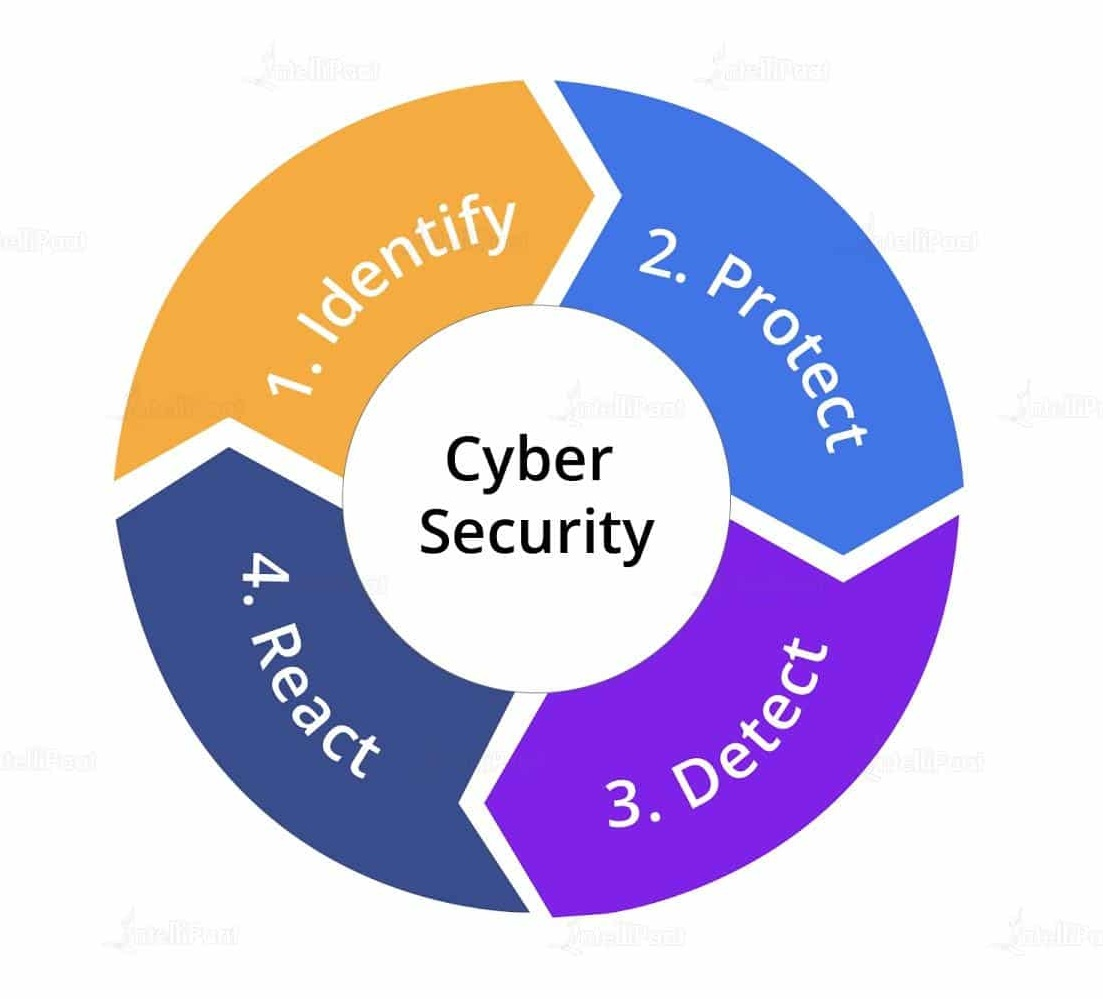
\includegraphics[scale=0.2]{faze.jpg}
	\end{center}
	\caption{Faze cybersecuritija}
\end{figure}




\newpage

\section{Hakovanje uopšteno}
\label{sec:hakovanje}
Termin haker se koristio za osobe koji su svojim znanjem i veštinama prepravljali sisteme i time povećavali njihovu efikasnost i dozvoljavali im da multi taskuju. 
Danas taj termin opisuje programere koji upadaju u sisteme tako što iskorišćavaju bagove i sigurnosne propuste.
Postoji tri različite grupe hakera i veoma je bitno napraviti razliku između njih. Uglavnom kada se govori o hakerima misli se na pojedince čije se radnje smatraju kriminalnim, ali postoje i oni drugi.

\begin{itemize}
\item \textbf{Etički hakeri ({\em White hat hacker})} - radnici kompanija koji imaju odgovarajuće znanje i koriste ga za dobrobit kompanije, odnosno omogućavaju kompaniji otpornost na hakere drugih vrsta. Glavna stvar koja ih razlikuje od ostalih vrsta hakera je to što oni imaju dozvolu kompanije za hakovanje. Vlasnici su ti koji su ih zaposlili i glavni cilj etičkih hakera je pronalaženje bezbednosnih propusta i mana u aplikacijama i sistemima.
\item \textbf{Zlonamerni hakeri ({\em Black hat hacker})} - pišu viruse i koriste ih kako bi upali u sisteme bez dozvole vlasnika sistema. Oni uglavnom kradu podatke i prodaju ih, pa su samim tim velika pretnja po sisteme. Rade ili pojedinačno ili u grupama i načini hakovanja postaju sve kreativniji iz godine u godinu. Mogu uništiti kompanije tako što objave poverljive podatke ili zahtevajući ogromne količine novca kako ne bi objavili te podatke.
\item \textbf{Hakeri iz sive zone ({\em Gray gat gacker})} - nešto između prethodna dva tipa, oni traže bezbednosne propuste i kada ih nađu oni obaveštavaju vlasnike sistema o njima i zahtevaju naknadu. Po tome su sličniji etičkim hakerima, samo je razlika u tome što oni nemaju dozvolu za traženje propusta, odnosno nisu zaposleni u tim kompanijama. A problem nastaje najčešće ukoliko vlasnik ne želi da plati naknadu, pa informacije o propustima ''isplivaju'' na površinu.
\end{itemize} \cite{ethackandcybersec}

"Postoje samo dva tipa kompanija: One koje su već hakovane i one koje će tek biti'' - Robert Mueller, direktor FBI
\newpage

\section{Etičko hakovanje}	
\label{sec:proces}
Pretpostavimo da ste napravili aplikaciju i primenili sve mere kako bi je zaštitili. Ali kako možete biti sigurni da je vaša aplikacija u potpunosti bezbedna i da niko ne može da zaobiđe sistem zaštite? Moraćete da proverite da li bilo koja od tehnologija ima sigurnosnih propusta u verziji koju ste koristili i da proverite da li mere zaštite u potpunosti funkcionišu. Upravo tu na scenu stupaju hakeri.

Etički hakeri istražuju sistem ili mrežu i traže slabe tačke koje mogu biti iskorišćene u nekom cyber napadu. Oni sakupljaju i analiziraju informacije kako bi pronašli način da sistem, mreža ili aplikacija budu bezbedni. Tim procesom se poboljšava sigurnost, a kao posledica sistem je otporniji na napade i neki napadi se mogu izbeći.

Oni između ostalog proveravaju:
\begin{itemize}
\item Injekcione napade
\item Promene u sistemu bezbednosti
\item Izloženost osetljivih podataka
\item Proboje autenfikacionih protokola
\item Komponente sistema i mreža koje mogu da se iskoriste kao pristupna tačka
\end{itemize}  \cite{whatisethacking}

\subsection{Injekcioni napadi}
 Pod injekcijom se smatra iskorišćavanje baga u softveru koji je prouzrokovan nevalidnim podacima, odnosno umetanjem koda koji će se izvršavati umesto nekog validnog unosa i time promeni tok izvršavanja softvera. U odnosu na mesto “injekcije” delimo ih na sql, xss, nativne (programske, sistemske) i druge.
 \begin{itemize}
 \item SQL ({\em Structured Query Language})  SQL je jezik koji služi za komunikaciju sa bazom podataka.
Napadač će pokušati da manipuliše upitom koji se pošalje bazi podataka i na taj način izvrši umetnute komande.
Pri uspešnom izvršavanju, dobija se odgovor u vidu tabele (osetljivih podataka korisnika, administratora ...)
\item XSS ({\em Cross-Site Scripting})  Ako aplikacija u svom ispisu podataka koristi nešto što joj korisnik upiše, otvara se prostor za ovaj tip napada. Kod koji je najčešće u JavaScript se ubaci pri ispisu i moguće je da on trajno promeni webstranicu ako ona nema dobru validaciju. Posledica je sajt koji može da prikuplja podatke od posetioca, menja kolačiće i dr.
\item Nativne ({\em Native}) Ako je napadač upoznat sa kodom i načinom izvršavanja programa ili sistema. On može da iskoristi to znanje i u delovima koji nisu najbolje obezbeđeni da ubaci svoj kod. Posledice mogu biti od blagih do totalne kontrole u zavisnosti od koda.
\end{itemize} \cite{injectionattacks}

\newpage
\subsection{Promene u sistemu bezbednosti}
 Svaka promena polise koja se tiče bezbednosti mora biti detaljno testirana kako bi se obezbedilo siguran rad aplikacije. Pod promenama u sistemu se smatra bilo šta što menja trenutni tok podataka
 
\subsection{Izloženost osetljivih podataka}
Pod osetljivim podacima, smatraju se svi oni podaci kojima se može identifikovati pojedinac. Etički haker će u ovom delu videti koliko su dobro čuvani podaci, odnosno koliko je jednostavno do njih doći. Jedan od načina bezbednog čuvanja podataka je da su podaci enkriptovani nekom metodom gde bi i u slučaju dobijanja tih podataka bilo neophodno dešifrovanje. 

\subsection{Proboje autenfikacionih protokola}
Autenfikacioni protokol je tip protokola koji služi za prenos podataka o autentifikaciji između servera i korisnika. Sastoji se od cetiri pravila koja se moraju poštovati: 
\begin{itemize}
\item Svi učesnici u protokolu znaju kakav je protokol
\item Ne sme se odstupati od protokola
\item Svaki korak protokola mora biti jasno definisan
\item Mora postojati akcija za svaki mogući scenario
\end{itemize}
\cite{authprotocolscrypto} \cite{authprotocolswiki}

\subsection{Komponente sistema i mreža koje mogu da se iskoriste kao pristupna tačka}
Pristupna tačka je bilo koja komponenta mreže ili sistema kroz koju svi korisnici moraju proći kako bi razmenili podatke. U kućnoj varijanti je to switch, ruter i wireless antena i da bi ste pristupili internetu vi morate proći kroz sve te uredjaje. Kod napada na pristupne tačke haker klonira jedan od tih uređaja i predstavlja se kao on. Postoje razne vrste napada u odnosu na način kloniranja: Man in the Middle (posrednik), Evil Twin (zli blizanac)...
\newpage

\section{Algoritam rada etičkog hakera}
\label{sec:algoritam}
Pronalaženje sigurnosnih propusta zahteva dosta vremena i strpljenja. Tipičan način rada zahteva od hakera da zaobiđe autorizacione i autentifikacione mehanizme, skenira mrežu i potraži sigurnosne greške. Proces je dodatno teži jer zlonamerni hakeri svakodnevno pronalaze nove načine za iskorišćavanje sigurnosnih procesa, pa se samim tim i način zaštite menja.
Da bi pronašli sigurnosne propuste, etički hakeri preduzimaju sledeće korake:
\begin{itemize}
\item \textbf{Izviđanje ({\em Reconnaissance})} - Pre nego što se sprovedu bilo kakvi testovi bezbednosnih propusta, mora se ''izvideti teren''. Izviđanje je pripremna faza u kojoj haker dokumentuje zahteve organizacije, pronalazi konfiguracione i pristupne informacije sistema i gleda od kojih delova se sastoji mreža. Neke od stvari koje su dokumentovane: servisi na mreži, serveri, IP adrese, imena i kredencijali osoba na mreži i fizičke logacije uređaja.
\item \textbf{Skeniranje ({\em Scanning})} - U ovoj fazi, skenira se mreža i identifikuju se potencijalne slabe tačke. Ovo uključuje skeniranje svih uređaja, korisnika, servisa unutar mreže korišćenjem automatskih alata za skeniranje. Ti alati sprovode tri tipa skeniranja, a to su:
\begin{itemize}
\item Mapiranje mreže  ({\em Network mapping})  - otkrivanje topologije mreže, informacija o serveru, ruterima i zaštitima unutar mreže. Kada se ovo završi može se vizualizovati mreža i napraviti plan o daljim postupcima.
\item Skeniranje portova  ({\em Port scanning}) - traženje otvorenih portova, enumeracija svih portova i servisa za koji se koriste kao i način konektovanja na te portove.
\item Skeniranje slabosti  ({\em Vulnerability scanning}) - korišćenje različitih alata koje proveravaju slabosti pojedinih verzija različitih tehnologija koje se koriste u mreži.
\end{itemize}
\item \textbf{Pristup ({\em Gaining access})} - kada se završi faza skeniranja, može se nastaviti sa pokušajem iskorišćavanja slabosti kako bi se dobile administratorske privilegije. To je najčešće slanje malicioznog koda aplikacijama kroz mrežu. Ukoliko su uspešni, imaju potpunu kontrolu celog ili dela sistema.
\item \textbf{Trajnost ({\em Maintaining access})} - akcije kojima se obezbeđuje trajnost pristupa u budućnosti, takođe u ovoj fazi se testira limit pristupa, odnosno proverava kolika je maksimalna kontrola koju haker može da ima na osnovu prethodnog pristupa. 
\item \textbf{Skrivanje ({\em Clearing track})} - da bi se sakrili tragovi koji pokazuju da je došlo do neovlašćenog pristupa mreži, hakeri moraju preduzeti neke akcije kao što su: brisanje skripta i aplikacija koje su korišćene za napade, promene vrednosti registra, čišćenje log fajlova i brisanje svih fajlova i foldera koje su nastale u toku napada.
\end{itemize}

Nakon što su svi koraci završeni, etički haker podnosi detaljan izveštaj i predlaže načine rešavanja sigurnosnih problema.
\cite{stepsethack}
\newpage

\section{Zaključak}
\label{sec:zakljucak}

Bezbednost nastavlja da bude velika briga svih tehnoloških kompanija i sve više se daje na značaju zaštiti poverljivih podataka. Ova briga proizilazi iz činjenice da su kritične tačke teške za pronalaženje i da je za pojedine propuste neophodno i do godinu dana za detekciju. Neophodno je razumeti potencijalne sigurnosne probleme kako na fizičkom nivou, tako i na aplikativnom. Shodno tome bezbednost mora pokriti ne samo neautorizovane pristupe mreži, nego i procese koje mogu smanjiti performanse ili unistiti mrežu u potpunosti.

Etičko hakovanje pomaže organizacijama da otkriju te propuste i da ih poprave pre nego što ih neko iskoristi. Kroz kombinaciju automatskih i manualnih testova, etički hakeri dostavljaju detaljan izveštaj bezbednosnih pretnji, efektivnost trenutnih bezbednosnih polisa i generalne savete za kreiranje bezbednih aplikacija.

\newpage

\addcontentsline{toc}{section}{Literatura}
\appendix

\iffalse
\bibliography{reference} 
\bibliographystyle{plain}
\fi

\begin{thebibliography}{11}

\bibitem{whatiscybersec} \href{https://www.itgovernance.co.uk/what-is-cybersecurity}{What is cybersecurity}
\bibitem{computersecurity} \href{https://en.wikipedia.org/wiki/Computer_security}{Computer security}
\bibitem{cyberphases} \href{https://www.etherwan.com/support/featured-articles/cyber-security-4-phases-creating-and-maintaining-secure-industrial-network}{Computer security}
\bibitem{ethackandcybersec} \href{https://www.wgu.edu/blog/ethical-hacking-how-fits-with-cybersecurity1908.html}{Ethical hacking and cybersec}
\bibitem{whatisethacking} \href{https://www.invicti.com/blog/web-security/what-is-ethical-hacking}{What is ethical hacking}
\bibitem{injectionattacks} \href{https://crashtest-security.com/what-are-the-different-types-of-injection-attacks}{Types of injection attacks}
\bibitem{authprotocolscrypto} \href{https://www.logsign.com/blog/what-are-authentication-protocols-in-cryptography/}{Authentication protocols in cryptography}
\bibitem{authprotocolswiki} \href{https://en.wikipedia.org/wiki/Authentication_protocol}{Authentication protocol wiki}
\bibitem{stepsethack} \href{https://crashtest-security.com/five-steps-of-ethical-hacking/}{Steps of ethical hacking}
\bibitem{ArtofExploration} Jon Erickson \emph{Hacking: The Art of Exploitation}, 2008
\bibitem{ThreatModeling} Adam Shostack \emph{Threat Modeling: Designing for Security}, 2014
\bibitem{CybersecurityEssentials} Charles J. Brooks, Christopher Grow, Philip Craig, and Donald Short \emph{Cybersecurity Essentials}, 2018

\end{thebibliography}

\end{document}